\section{歪曲収差以外の収差とその特徴について}
1章にて、収差には単色収差と色収差が存在すると述べた。また、単色収差にはザイデルの5収差がある。
\subsection{ザイデルの5収差}
\subsubsection{球面収差}
球面収差とは、レンズ面が球面であることにより発生する収差である。ここで、\eqref{seidelx},\eqref{seidely}から球面収差の項のみを考える。つまり、
\begin{eqnarray}
	\Delta x' & = & A r^3 \sin \theta \\
	\Delta y' & = & A r^3 \cos \theta
\end{eqnarray}
以上の式より、球面収差は入射高の3乗に比例し、像の高さに依存しない。口径を絞り込むことによって収差は少なくなるといえる。
%球面収差とは、光軸から離れた光線ほど、光学系浸透後に、軸上での像点が手前にできてしまうことをいう。他の収差と異なり、像面全体に同量の収差を生じさせる。また光軸上の物体に対しても収差が存在するのは、球面収差だけとなってである。
\begin{figure}[h]
	\centering
	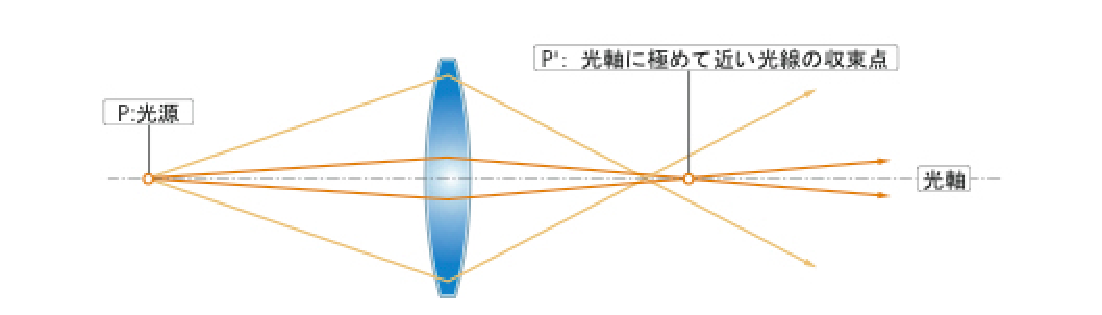
\includegraphics[height=30mm]{image/kyumen.png.eps}
	\caption{球面収差\ \cite{cite1}}
	\label{caption1}
\end{figure}
\subsubsection{コマ収差}
コマ収差とは、光軸より離れた物点の横倍率が物点の位置により異なる収差のことをいう。ここで、\eqref{seidelx},\eqref{seidely}からコマ収差の項のみを考える。つまり、
\begin{eqnarray}
	\Delta x' & = & B r^2 y\sin 2 \theta \\
	\Delta y' & = & B r^2 y (2+\cos 2\theta)
\end{eqnarray}
以上の式より、コマ収差は入射高の2乗に比例し、像高に比例する。つまり、口径を絞り込むことによって収差は少なくなるといえる。
\begin{figure}[h]
	\centering
	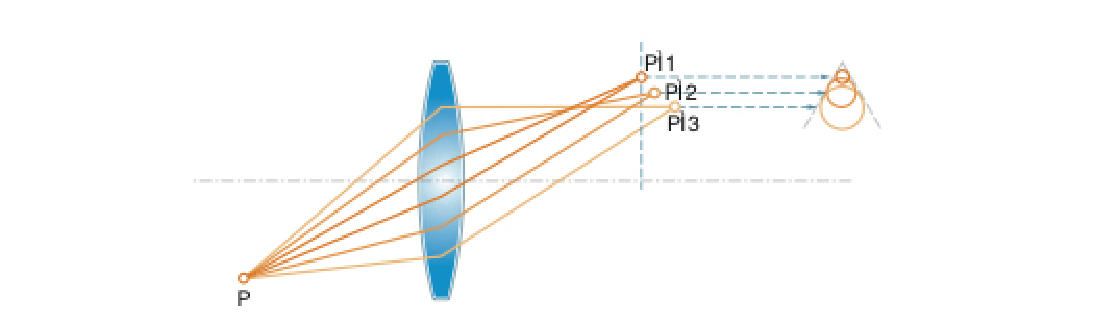
\includegraphics[height=30mm]{image/koma.png.eps}
	\caption{コマ収差\ \cite{cite1}}
	\label{caption1}
\end{figure}
\vspace{10cm}
\subsubsection{非点収差と像面収差}
非点収差とは、子午光線と球欠光線に対する焦点距離の違いのことをいう。
像面収差とは、光軸に平行な光線と傾いた光線が、光軸に垂直な同一面に結像しないことをいう。
ここで、非点収差と像面収差の項を考える。したがって、
\begin{eqnarray}
	\label{seidelx}
	\Delta x' & = & D r y^2 \sin \theta \\
	\label{seidely}
	\Delta y' & = & (2C+D)r y^2 \cos \theta 
\end{eqnarray}
以上の式から、どちらの収差も、入射高に比例し、像高の2乗する。また、
像面収差は非点収差と異なり、湾曲も起こる。
\begin{figure}[h]
	\centering
	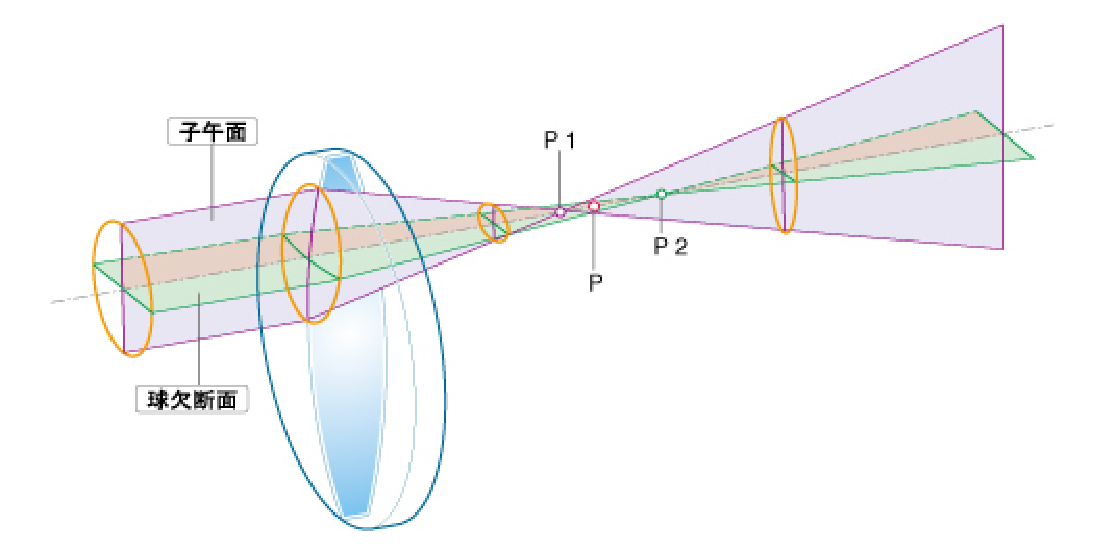
\includegraphics[height=40mm]{image/hiten.png.eps}
	\caption{非点収差\ \cite{cite1}}
	\label{caption1}
\end{figure}
\begin{figure}[h]
	\centering
	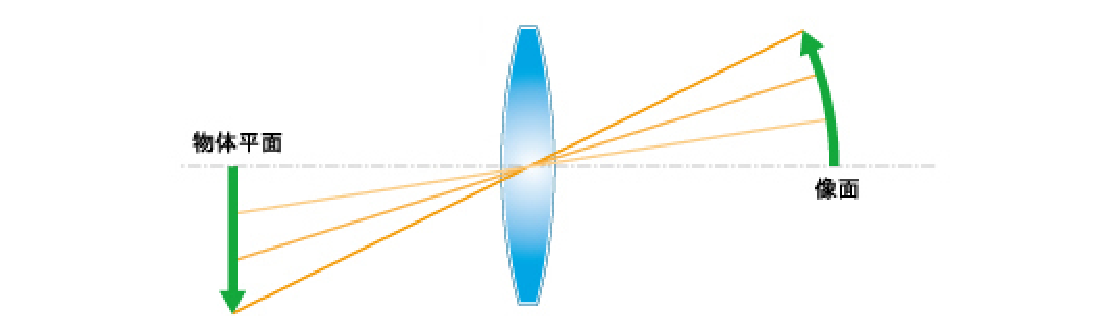
\includegraphics[height=30mm]{image/zomen.png.eps}
	\caption{像面収差\ \cite{cite1}}
	\label{caption1}
\end{figure}

\subsection{色収差}
\subsubsection{軸上色収差}
軸上色収差とは、光の波長によって光軸上で結像位置が異なる収差のことをいう。凸レンズと凹レンズを組み合わせることによって防ぐことができる。
\begin{figure}[h]
	\centering
	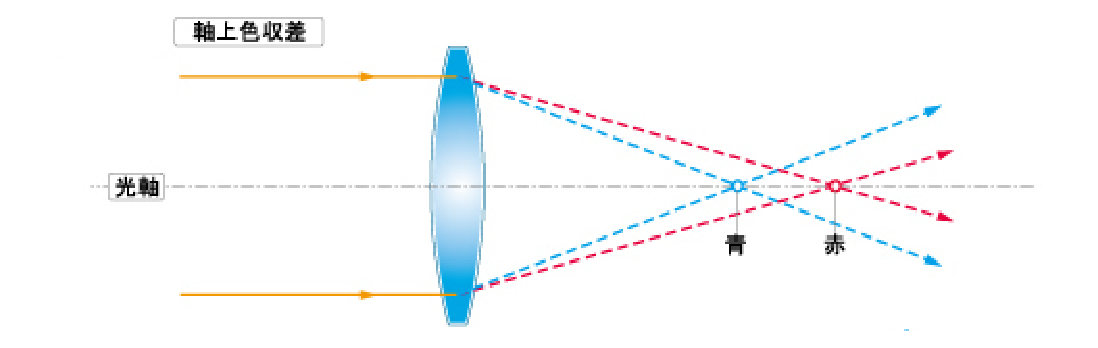
\includegraphics[height=30mm]{image/jikujo.png.eps}
	\caption{軸上色収差\ \cite{cite1}}
	\label{caption1}
\end{figure}
\subsubsection{倍率色収差}
倍率色収差とは、光の波長によって像の大きさが異なる収差のことをいう。この像の大きさの違いは波長による屈折率が異なることによって生じる。波長の像倍率の補正を行うことによって収差を防ぐことができる。
\begin{figure}[h]
	\centering
	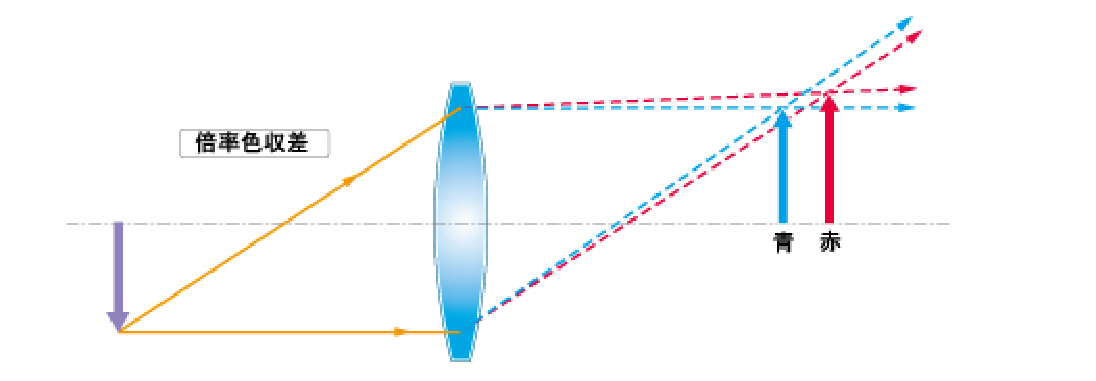
\includegraphics[height=30mm]{image/bairitsu.png.eps}
	\caption{倍率色収差\ \cite{cite1}}
	\label{caption1}
\end{figure}